% This file was created with tikzplotlib v0.9.12.
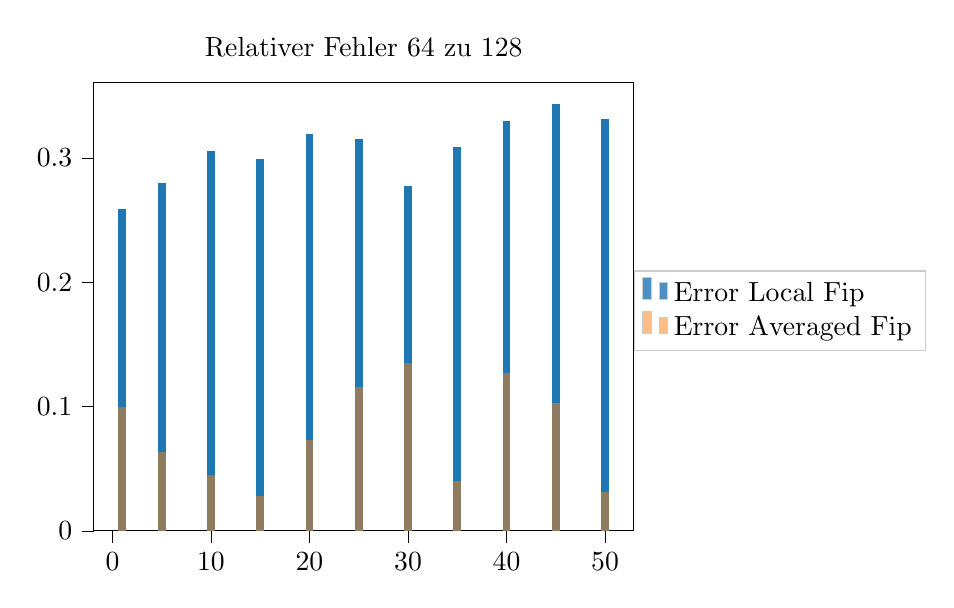
\begin{tikzpicture}

\definecolor{color0}{rgb}{0.12156862745098,0.466666666666667,0.705882352941177}
\definecolor{color1}{rgb}{1,0.498039215686275,0.0549019607843137}

\begin{axis}[
legend cell align={left},
legend style={
  fill opacity=0.8,
  draw opacity=1,
  text opacity=1,
  at={(1,0.4)},
  anchor=south west,
  draw=white!80!black
},
tick align=outside,
tick pos=left,
title={Relativer Fehler 64 zu 128},
x grid style={white!69.0196078431373!black},
xmin=-1.89, xmax=52.89,
xtick style={color=black},
y grid style={white!69.0196078431373!black},
ymin=0, ymax=0.360761981864844,
ytick style={color=black}
]
\draw[draw=none,fill=color0] (axis cs:0.6,0) rectangle (axis cs:1.4,0.258970966587948);
\addlegendimage{ybar,ybar legend,draw=none,fill=color0}
\addlegendentry{Error Local Fip}

\draw[draw=none,fill=color0] (axis cs:4.6,0) rectangle (axis cs:5.4,0.280080867138823);
\draw[draw=none,fill=color0] (axis cs:9.6,0) rectangle (axis cs:10.4,0.305690899026233);
\draw[draw=none,fill=color0] (axis cs:14.6,0) rectangle (axis cs:15.4,0.299383127260441);
\draw[draw=none,fill=color0] (axis cs:19.6,0) rectangle (axis cs:20.4,0.319251681760401);
\draw[draw=none,fill=color0] (axis cs:24.6,0) rectangle (axis cs:25.4,0.314928430182427);
\draw[draw=none,fill=color0] (axis cs:29.6,0) rectangle (axis cs:30.4,0.277160472130012);
\draw[draw=none,fill=color0] (axis cs:34.6,0) rectangle (axis cs:35.4,0.308483591219375);
\draw[draw=none,fill=color0] (axis cs:39.6,0) rectangle (axis cs:40.4,0.329944321530422);
\draw[draw=none,fill=color0] (axis cs:44.6,0) rectangle (axis cs:45.4,0.34358283987128);
\draw[draw=none,fill=color0] (axis cs:49.6,0) rectangle (axis cs:50.4,0.331086673399495);
\draw[draw=none,fill=color1,fill opacity=0.5] (axis cs:0.6,0) rectangle (axis cs:1.4,0.0992355412113805);
\addlegendimage{ybar,ybar legend,draw=none,fill=color1,fill opacity=0.5}
\addlegendentry{Error Averaged Fip}

\draw[draw=none,fill=color1,fill opacity=0.5] (axis cs:4.6,0) rectangle (axis cs:5.4,0.0631194785990044);
\draw[draw=none,fill=color1,fill opacity=0.5] (axis cs:9.6,0) rectangle (axis cs:10.4,0.0451151303669287);
\draw[draw=none,fill=color1,fill opacity=0.5] (axis cs:14.6,0) rectangle (axis cs:15.4,0.0283429433787608);
\draw[draw=none,fill=color1,fill opacity=0.5] (axis cs:19.6,0) rectangle (axis cs:20.4,0.0728691336881973);
\draw[draw=none,fill=color1,fill opacity=0.5] (axis cs:24.6,0) rectangle (axis cs:25.4,0.11604532747568);
\draw[draw=none,fill=color1,fill opacity=0.5] (axis cs:29.6,0) rectangle (axis cs:30.4,0.134661520078081);
\draw[draw=none,fill=color1,fill opacity=0.5] (axis cs:34.6,0) rectangle (axis cs:35.4,0.0402080045082676);
\draw[draw=none,fill=color1,fill opacity=0.5] (axis cs:39.6,0) rectangle (axis cs:40.4,0.127242864120504);
\draw[draw=none,fill=color1,fill opacity=0.5] (axis cs:44.6,0) rectangle (axis cs:45.4,0.102508324774774);
\draw[draw=none,fill=color1,fill opacity=0.5] (axis cs:49.6,0) rectangle (axis cs:50.4,0.0313606243706717);
\end{axis}

\end{tikzpicture}
